\documentclass[sigconf,review=false]{acmart}
\usepackage{pdfpages}
\usepackage{hyperref}
\usepackage{booktabs}
\usepackage{pdflscape}
\usepackage{caption}
\usepackage{longtable}

\renewcommand\footnotetextcopyrightpermission[1]{}
\settopmatter{printacmref=false, printccs=false, printfolios=false}
\acmConference[University of Cape Town]{University of Cape Town}{Cape Town, South Africa}{2026}
\acmBooktitle{}
\acmPrice{}
\acmDOI{}
\acmISBN{}
\setcopyright{none}
\title{Does Hierarchy Help? Few-Shot Adaptation of Feudal and Flat Policies in Real-Time Strategy Games}

\author{Conor Karl McKeag}
\affiliation{
  \institution{University of Cape Town}
  \city{Cape Town}
  \country{South Africa}
}
\email{mckcon007@myuct.ac.za}

\date{08 August 2026}

\begin{document}

\begin{abstract}
Hierarchical reinforcement learning (HRL) promises the temporal
abstraction, sample efficiency, and transfer ability that real-time
strategy (RTS) games demand, yet no HRL method has been evaluated in
a full-game RTS setting. We address this gap with FeudalNet, a
hierarchical Gym-\textmu RTS agent retaining the Manager/Worker
division of FeUdal Networks but replacing its recurrent memory with
dual-timescale transformers and adding a dedicated
opponent-modelling stream. We evaluate FeudalNet alongside
TransformerNet, a state-of-the-art flat policy, on few-shot
adaptation: a fully-trained agent trains against an unseen opponent
until a 90\% win-rate or a 1M-step cap (versus 300M for training),
and the change in win-rate is measured. FeudalNet defeats all
fourteen scripted opponents in round-robin play and exceeds
TransformerNet on the standard evaluation suite, including an
88.2\% win-rate against coacAI. Under adaptation, FeudalNet improved
significantly against all four unseen opponents, lifting its weakest
matchup from 42.8\% to 95.5\% via a discovered counter-strategy,
while TransformerNet improved against one, held level against two,
and regressed against one; FeudalNet's adaptation score was
significantly higher on three of four. These results answer the
research question affirmatively and suggest the hierarchy's
advantage lies not only in how much it adapts but in how reliably,
requiring less intervention than the flat baseline.
\end{abstract}

\maketitle

\section{Introduction}
Real-time strategy (RTS) games remain one of the most demanding challenge domains for reinforcement learning (RL). An agent must manage economy, production, and combat simultaneously, over combinatorial action spaces in which every unit on the board acts at every tick. Additionally, these games often provide only a terminal win or loss signal, over horizons spanning thousands of steps. 
Flat deep RL has conquered these games at the highest level - AlphaStar reached grandmaster rating in StarCraft II~\cite{alphastar} and OpenAI Five defeated world champions in Dota~2~\cite{dota2five}. 
Both, however, required training infrastructure beyond the reach of most research groups. 
The Gym-$\mu$RTS environment~\cite{micrortsgridnet} was developed specifically to close this infrastructure gap, enabling full-game RTS research on a single machine, and has since accumulated a family of strong flat-policy agents~\cite{micrortsgridnet, transformernet}.

Hierarchical reinforcement learning (HRL) is, on paper, a natural fit for the difficulties RTS games pose. By splitting decision-making into a high-level policy that selects goals on a long timescale and a low-level policy that executes primitive actions on a shorter one, HRL shortens the credit-assignment horizon and converts sparse extrinsic rewards into dense intrinsic ones for the low-level policy. 
This mirrors the division between strategy and micro-management that RTS games demand of human players. Yet despite this apparent fit,
HRL methods have not been evaluated in a full-game RTS setting.
FeUdal Networks (FuN)~\cite{FuN} was evaluated on Atari, and subsequent hierarchical methods have been largely confined to navigation and manipulation benchmarks. Whether the promised benefits of temporal abstraction - sample efficiency, strategic credit assignment and, in particular, the ability to transfer to unseen tasks, and to do so reliably - also appear in a full RTS game remains an open empirical question.

This paper addresses that gap. We introduce FeudalNet, a hierarchical agent for Gym-$\mu$RTS that retains the Manager/Worker division of FuN but replaces the recurrent memory at both levels with transformers operating on different timescales, augmented with a dedicated opponent-modelling stream. 
We evaluate it alongside TransformerNet~\cite{transformernet}, a state-of-the-art flat policy, on a task chosen to probe the transfer claim directly, which we refer to as few-shot adaptation. 
A fully-trained agent is granted a small additional training budget against a previously unseen opponent - training until it reaches a 90\% win-rate or a cap of 1M steps, against 300M for initial training - and the change in win-rate is measured. Hence, we ask the following research question: \emph{Given a limited adaptation budget, does the hierarchical FeudalNet agent improve its win-rate against unseen opponent strategies in Gym-$\mu$RTS by more than the flat TransformerNet agent?}

Our contributions are threefold. 
First, we present, to our knowledge, the first evaluation of a feudal HRL architecture in a full-game RTS environment, together with the architectural modifications needed to make the feudal structure work in a spatial, multi-unit action space. 
Second, we establish baseline strength - FeudalNet defeats all fourteen scripted opponents in a round-robin setting more convincingly than any scripted contender and exceeds TransformerNet on the standard evaluation suite, including an $88.2\%$ win-rate against coacAI, the baseline used in most of the literature. 
Finally, we answer the research question by comparing both agents under the few-shot adaptation procedure against four unseen opponents selected for difficulty. 
FeudalNet improves significantly against all four, in one case discovering a new counter-strategy that turns its weakest matchup into a near-solved one, whereas TransformerNet improves significantly against only one and regresses against another. 
Beyond the magnitude of adaptation, we find that the hierarchy adapts far more reliably, requiring minimal intervention where the flat baseline proved sensitive to nearly every choice made in adapting it - a result we did not set out to test but regard as the most notable of the study.

The remainder of this paper is structured as follows.
Section~\ref{relatedworks} reviews related work in HRL and RTS-based RL. 
Section~\ref{methods} details the environment, both agent architectures, the evaluation process and the adaptation procedure.
Section~\ref{results} presents results and their interpretation, and
Section~\ref{conclusions} concludes with directions for future work.

\section{Related Work}
\label{relatedworks}

Real-time strategy (RTS) games are among the most demanding testbeds for reinforcement learning: action spaces are combinatorial (approximately $10^8$ possibilities per action in StarCraft II), rewards are sparse and often granted only at a win or loss, matches span long horizons, and opponents are strategically diverse. 
Flat deep RL has succeeded in these settings - AlphaStar \cite{alphastar} and OpenAI Five \cite{dota2five} - but only at a computational scale unavailable to most researchers.

Hierarchical reinforcement learning (HRL) directly targets these difficulties. 
A high-level policy selects sub-tasks over a coarse timescale while a low-level policy executes primitive actions over a fine one, shortening the effective task horizon through temporal abstraction.
Since the low level is trained on intrinsic rewards for reaching sub-goals while only the high level consumes the extrinsic signal, HRL is naturally suited to sparse-reward problems, and has been shown to require 3–5x fewer environment interactions \cite{HAC, badhrl} than flat RL.

Of the deep HRL methods reviewed, FeUdal Networks (FuN) \cite{FuN} is the most relevant to this work. 
A Manager operating at low temporal resolution - implemented as a novel dilated LSTM - emits goals as directions in a learnt latent state-space, and a Worker produces primitive actions, intrinsically rewarded by the cosine similarity between its state change and the goal direction. 
The Manager is trained purely on extrinsic reward, so goal discovery is not reduced to Worker management. 
FuN learnt meaningful sub-goals in the Atari domain, including sparse-reward Montezuma's Revenge, and transferred effectively between games - a property relevant to adapting against unseen RTS opponents - though it exhibited long stagnation periods, suggesting difficulty finding optimal sub-policies. 
Two further methods illustrate complementary mechanisms: Hierarchical Actor-Critic \cite{HAC} stabilises the parallel learning of multiple policy levels by training each level with hindsight as though the levels below were already optimal, and Hierarchical Decision Transformers \cite{DT-HRL} recast the hierarchy as conditional sequence modelling, relabelling high-return trajectory states as sub-goals; HDT excelled on long-horizon, sparse-reward tasks and could gain few-shot adaptation through online fine-tuning.

Gym-$\mu$RTS \cite{microrts, micrortsgridnet} makes full-game RTS research affordable, training state-of-the-art agents on a single GPU. 
Observations are (h, w, 27) feature tensors; the variable action space is decomposed into a unit action space of 8-dimensional discrete vectors and a player action space issuing these per unit. Two policy schemes were compared: UAS, which iterates over units, and Gridnet, which predicts actions for every cell in one step.
Their experiments established that invalid action masking is indispensable (without it, a 0\% win rate) and that a diverse opponent pool during training is necessary to avoid losses to simple rush strategies; the best agent, UAS, reached a 91\% cumulative win rate. 
TransformerNet \cite{transformernet} later replaced Gridnet's dense grid with per-entity feature vectors processed by a 5-layer, 7-head transformer encoder, achieving better reward maximisation (189.7 vs 137.6) and faster training - but a lower win rate, traced to reward hacking in which the agent crippled opponents to farm shaped rewards, indicating the win/loss weight was set too low.

An important caveat spans this literature: HRL results are largely empirical, and Nachum et al. \cite{badhrl} show much of the benefit may stem from improved exploration, with well-explored flat RL sometimes matching HRL. 
Fair evaluations therefore require flat baselines equipped with strong exploration. 

Overall, HRL's temporal abstraction, sample efficiency, and transfer ability make it well matched to RTS games, yet no HRL method has been evaluated in a full-game RTS setting - a gap this work addresses using Gym-$\mu$RTS as the platform.

\section{Methods}
\label{methods}
All code, trained models and raw results for the experiments described in this section are available in our GitHub repository.\footnote{\url{https://github.com/rhatos/FeudalNet}}
\subsection{Environment \& Task}

\subsubsection{$\mu$RTS Environment}

The $\mu$RTS \cite{microrts} environment is an implementation of a simple RTS game designed to perform lightweight AI research.
The objective is to destroy the opponent's base and all of their units.
In order to achieve this, one must gather resources, create units and command them to attack the enemy.

\subsubsection{Map Sizes}
Our evaluation used two map sizes, $8 \times 8$ and $16 \times 16$ (Figure~\ref{fig:map-sizes}), as each demands a different style of play. 
On the $8 \times 8$ map, a ``rush'' strategy - in which the player rapidly produces worker units and immediately sends them to attack - is generally considered optimal, since the confined space leaves little room for alternative approaches. 
In contrast, no single strategy dominates on the $16 \times 16$ map: its larger size renders a basic rush insufficient and rewards more deliberate play. 
Larger map sizes were not considered due to the increased compute time they would require.

\begin{figure}
    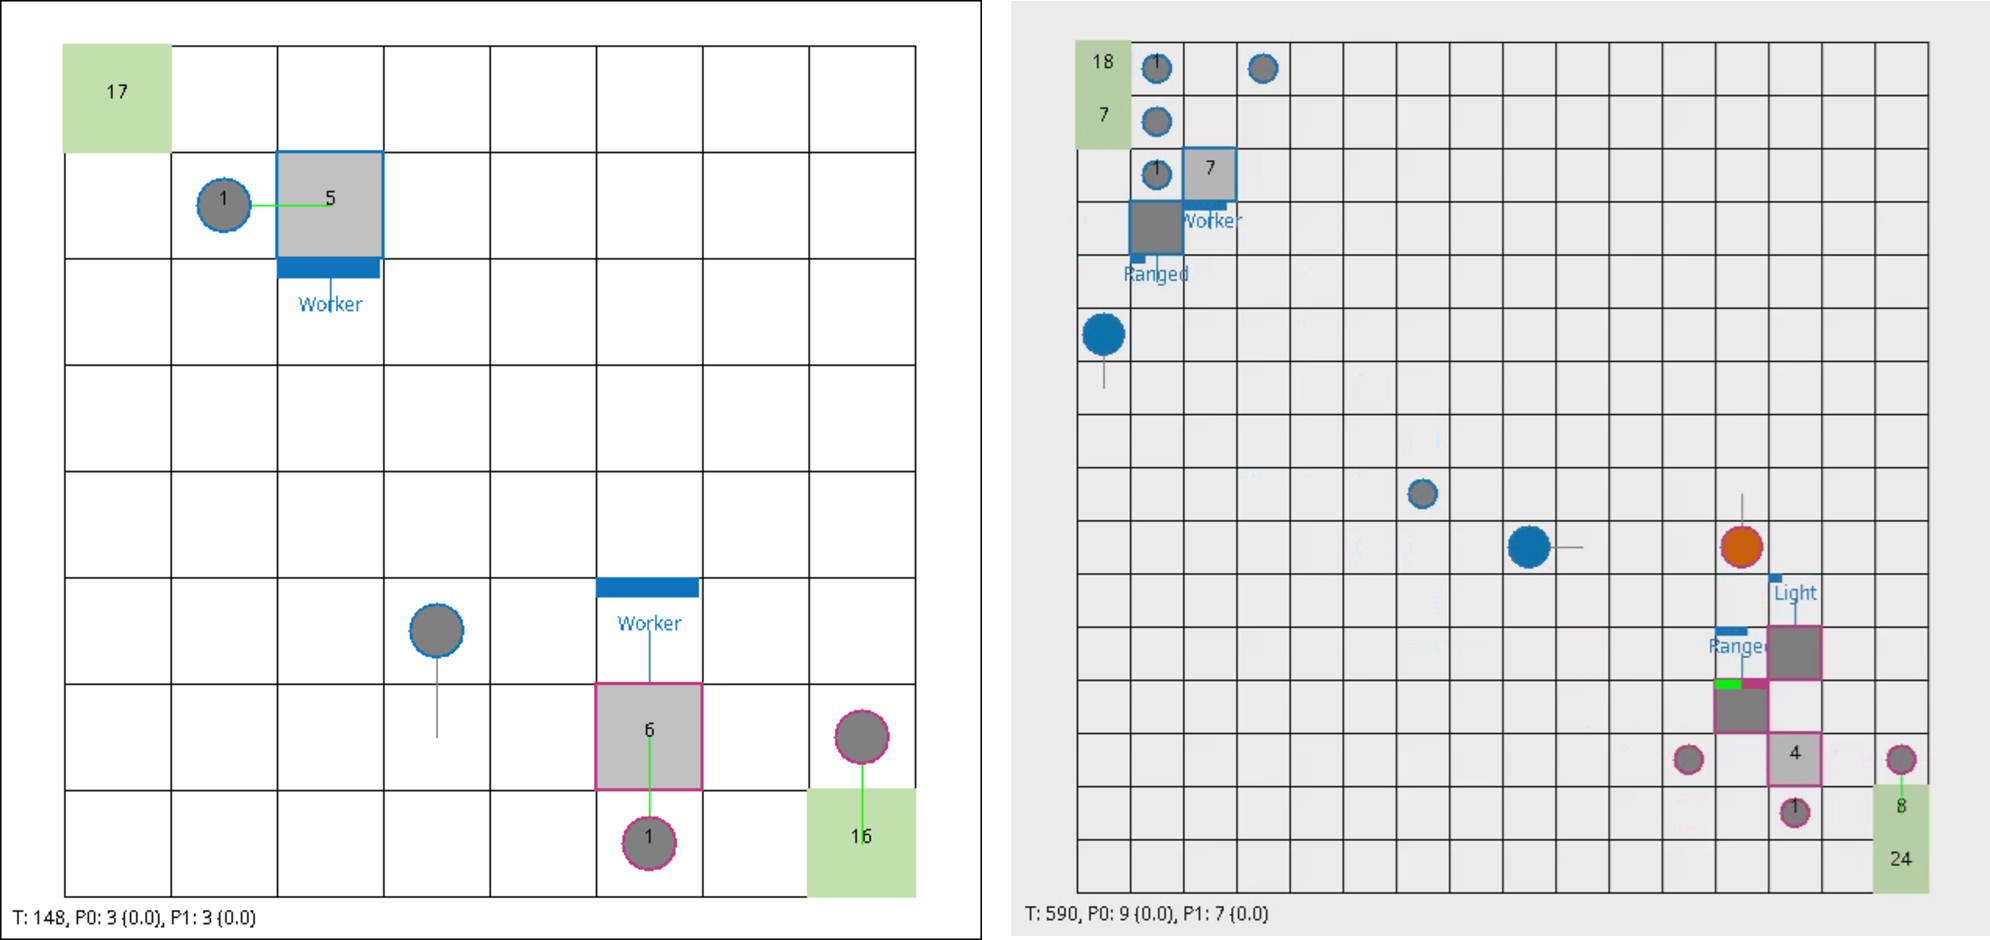
\includegraphics[width=0.45\textwidth]{./8x8v16x16.pdf}
    \caption{Left: 8x8 map, right: 16x16 map}\label{fig:map-sizes}
\end{figure}

\subsubsection{Game Conditions}
Each evaluation game is played under the following conditions: a win requires destroying all enemy units and buildings, while a loss occurs when all of one's own units and buildings are destroyed. 
If no victor has been declared after $2000$ game ticks, the game is ruled a draw; in our evaluation, draws are counted as losses.

\subsubsection{Opponents}
We evaluated against $14$ scripted opponents, all sourced from the
$\mu$RTS repository. Notable among them are
mayari\footnote{\url{https://github.com/barvazkrav/mayariBot}}
(winner of the 2021 CoG competition and runner-up in 2024),
coacAI\footnote{\url{https://github.com/Coac/coac-ai-microrts}}
(winner of the 2020 CoG competition), and
tiamat\footnote{\url{https://github.com/jr9Hernandez/TiamatBot}}
(winner of the 2018 CIG competition), with standings for all years
published by the competition
organisers.\footnote{\url{https://sites.google.com/site/micrortsaicompetition/competition-results}}
The full list of opponents is given in Table~\ref{tab:opponent-table}.
Of these, coacAI, workerRushAI, lightRushAI, and randomBiasedAI were
used during training.

\subsection{Agent Architectures}

The following section presents a high-level overview of each agent's architectures.

\subsubsection{FeudalNet Architecture}

FeudalNet is a hierarchical agent for Gym-\textmu RTS that retains the Manager/Worker division of FeUdal Networks (FuN) \cite{FuN} but replaces the recurrent memory at both levels with transformers operating on different timescales.
A shared IMPALA-style \cite{impala-cnn} residual CNN (the Perception module) encodes each observation without pooling and emits two representations from a single pass: a global embedding $z$ that feeds both hierarchy levels, and the pre-flatten spatial feature map that feeds the actor so that per-cell action logits are computed from local context. 
In parallel, an Enemy Encoder reduces each cell's enemy planes to a type identifier, embeds them position-wise, and accumulates opponent behaviour through a stacked LSTM; its output is fused into the Manager alone.

The Manager operates on a dilated clock, computing a new goal only every $c$ steps via a pre-norm transformer over a window of $T_M$ Manager states (spanning $T_M \times c$ environment steps), and emits an $L_2$-normalised goal direction trained by advantage-weighted cosine similarity between the goal and the subsequent latent state transition.
The Worker acts every step: its own transformer attends over the last $T_W$ embeddings, while a ConvTranspose decoder - over the pre-flatten spatial feature map - produces per-cell logits split into seven masked multi-discrete heads. 
The Manager's influence enters solely as a projected goal bias added uniformly to these logits and an intrinsic cosine reward encourages the Worker to follow the proposed direction, similar to that found in the original FuN \cite{FuN} paper. 

Both levels maintain separate critics and discounts, with a PPG-style \cite{PPG} auxiliary phase retraining the Worker's value head on stored hidden states.
A diagram demonstrating each component is shown in Figure~\ref{fig:feudalnet-architecture}.

\begin{figure*}[t]
    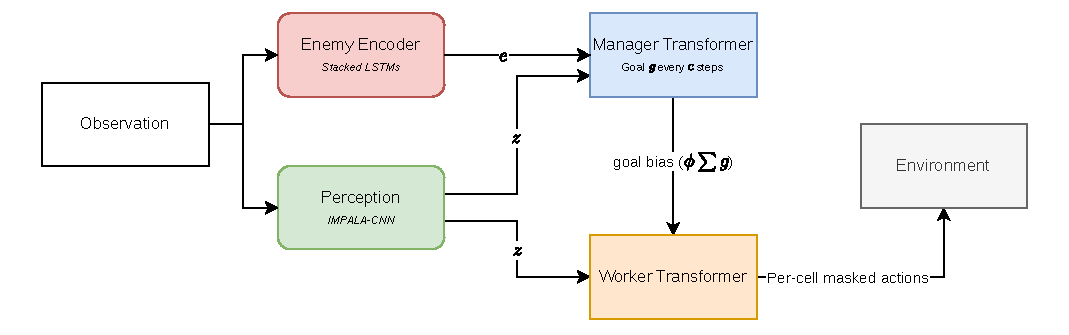
\includegraphics[width=0.9\textwidth]{./feudalnet_diagram.pdf}
    \caption{High-level overview of the FeudalNet architecture.}\label{fig:feudalnet-architecture}
\end{figure*}

\subsubsection{TransformerNet Architecture}

TransformerNet~\cite{transformernet} is a flat, entity-centric policy for Gym-\textmu RTS: unlike FeudalNet, it employs no hierarchical decomposition, temporal abstraction, or opponent-modelling stream - a single policy maps observations directly to unit actions at every step. 
A feature map $\phi(s_t)$ first converts the grid observation into a variable-length set of $e_t$ entity representations (one per friendly, enemy, and neutral unit), each formed by concatenating the entity's one-hot grid position with its 27-dimensional feature vector; on larger maps the positional one-hot is compressed through a trainable embedding so the representation size is invariant to board dimensions. 
These entity tokens are processed by a five-layer transformer encoder with seven attention heads and no positional encoding, whose self-attention naturally accommodates the variable number of units on the board.

The actor applies a single shared feed-forward layer to each encoded token belonging to an agent-controlled unit, yielding per-unit multi-discrete sub-action logits (78 per unit, with invalid actions masked) - so logits are produced only for cells that actually contain controllable units, avoiding GridNet's wasted computation on empty cells \cite{micrortsgridnet} while remaining model-free, unlike Unit Action Simulation (UAS). 
The critic scores every entity token, aggregates the per-entity values into sum and mean statistics per owner (agent, opponent, neutral), and combines these six metrics through a final learned layer into a single value estimate invariant to unit count. 
Trained with PPO under shaped rewards against scripted opponents, TransformerNet matched or exceeded prior Gym-\textmu RTS agents at roughly half the training cost of GridNet, though its purely reactive, single-timescale design leaves long-horizon strategic credit assignment entirely to the flat policy.

\subsection{Training}
\label{Training}

This section gives a high-level overview of the training conditions used for our FeudalNet agent.
We do not include TransformerNet training details as we used the best model found by Zwingenberger \cite{transformernet} for our evaluation of this agent.

\subsubsection{Seen Opponents}

We used 48 environment instances for training in parallel.
Where, 12 of these instances were reserved for each opponent used.
The following opponents were used:

\begin{itemize}
    \item coacAI
    \item workerRushAI
    \item randomBiasedAI
    \item lightRushAI
\end{itemize}

These four opponents follow the trends found in the literature \cite{transformernet, micrortsgridnet}.
Specifically, it has been found that a diverse opponent pool offers richer learning \cite{micrortsgridnet} and without it can result in very poor performance.

\subsubsection{Training Parameters}
% GAME LENGTH
We trained the FeudalNet agent for a total of $300$M in-game ticks.
It should be noted that this differs from the literature which commonly uses $100$M in-game ticks.
This was done after finding that $100$M ticks was not enough experience for the hierarchy to learn effectively.
Specifically, the highest win-rate achieved against coacAI after $100$M ticks was only $37$\% on the $16\times 16$ map.

% LEARNING RATE
The learning rate used was $4\times10^{-4}$ with a cosine-anneal applied.
We found during training that the agent would learn primitive actions very quickly such as creating workers and harvesting resources, but still needed more training to learn how to win games.
Hence, we used a cosine-anneal to encourage learning the primitive actions and then not easily forget them afterwards.

% TW TM C
We set the Worker's attention window ($\texttt{T\_W}$) to $100$ environment ticks.
Thus, the Worker's decisions directly reference anything that occurred in the last $100$ ticks. 
For the Manager, we set the attention window ($\texttt{T\_M}$) to $160$ steps.
Additionally, we set the Manager's time horizon ($\texttt{c}$) to $25$ (Update every $25$ ticks).
Hence, the Manager can reference $\texttt{T\_M} \times c$ environment steps of history.

The full list of hyperparameters can be found in Table~\ref{tab:hyperparams}.

\subsubsection{Reward Structure}
\label{reward-struct}
% REWARD STRUCTURE
Similar to the literature we made use of a shaped reward structure.
Specifically:

\begin{itemize}
    \item $+20$ for a win, $-20$ for a loss, $+0$ for a draw ($2000$ in-game ticks).
    \item $+1$ for harvesting one resource, $+1$ for producing one worker, $+0.2$ for constructing a building.
    \item $+1$ for each valid attack action issued, $+4$ for each combat unit produced.
\end{itemize}

The only change made to the reward structure found in the literature was increasing the reward/penalty for a win/loss from $\pm10$ to $\pm20$.
It was found by Zwingenberger \cite{transformernet} that a reward of $\pm10$ was too low and resulted in their agent occasionally not prioritising winning over all other actions.
Thus, we increased this reward and did not find the same behaviour in our agent.

\subsection{Parameter Tuning}
\label{param-tuning}
No systematic hyperparameter search was performed; the values in Tables~\ref{tab:feudalnet-hyperparameter-change} and~\ref{tab:hyperparams} were set manually over the course of development.
The general PPO training parameters (discount factors, GAE $\lambda$, entropy and value-loss coefficients, and gradient clipping) were taken as starting points from the Gym-$\mu$RTS agents of Huang et al.~\cite{micrortsgridnet}, the only published settings for full-game $\mu$RTS training, and adjusted only where manual test runs showed a need.
The hierarchy-specific parameters - the Manager horizon $c$, the attention windows $T_M$ and $T_W$, the intrinsic reward weight, and the PPG cadence - have no precedent at this scale, and the values reported by FuN~\cite{FuN} and PPG~\cite{PPG} were not adopted as they target very different domains.
These were instead chosen through short manual test runs on the $16\times16$ map against the training opponents, retaining values that produced stable learning; the resulting choices of step budget, learning-rate schedule and attention windows are justified in Section~\ref{Training}.

Adaptation hyperparameters were fixed from analysis of each agent's training run before any adaptation was attempted and were never revised in response to adaptation results (Section~\ref{adaptation-selection}).
TransformerNet was used with the published values of Zwingenberger~\cite{transformernet}.
Full details of the test runs and the values tried are provided in the online repository.

\subsection{Metrics \& Analysis}

The following section lists and discusses the three metrics being reviewed for our conclusions.
These metrics are used to compare each agent to each other directly.

\subsubsection{Adaptation}

Our primary metric is "adaptation", which we define as: for agent $a$ and unseen opponent $o$, the adaptation score is $\Delta_{a,o} = \text{WR}^{post}_{a,o} - \text{WR}^{pre}_{a,o}$, where each win-rate is measured over 1000 evaluation games.
We use $\Delta_{\text{FeudalNet}, o}$ against $\Delta_{\text{TransformerNet}, o}$ to directly answer the primary research question.
This value evaluates the agent's ability to achieve few-shot adaptation.
However, it should be noted that each agent starts at different win-rates for each opponent.
In order to counteract this, we report relative improvement normalised by the amount of room to improve, $\Delta_{a,o}/(1-\text{WR}_{a,o}^{\text{pre}})$, along with the raw delta.

Since each win-rate is a proportion estimated from a finite sample of games, an observed adaptation score can be non-zero purely by chance: at 1000 games per condition, differences of a few percentage points fall within the sampling variability of the measurement itself.
To distinguish genuine adaptation from noise, we test each adaptation score with a two-proportion z-test, which asks whether the pre- and post-adaptation win-rates could plausibly have been drawn from the same underlying win probability. 
This test is the appropriate choice here because the two conditions are independent samples of binary outcomes (win or loss) of equal size, which is exactly the setting the test assumes. 
Only adaptation scores that are significant at the 5\% level are treated as evidence of adaptation when answering the research question; scores that fail the test are reported but regarded as indistinguishable from no change.

\subsubsection{Steps to Win \& Lose}

A secondary metric which will be analysed is the mean game length in ticks over winning and losing games, measured pre- and post-adaptation.
Specifically, we ask whether the agent has learned to win quicker and lose slower as well as discussing any outliers.
A quicker win would imply that the policy has found and is exploiting a weakness; longer losses suggest improved defensive play even when the matchup is not won yet.
However, adaptation converts former losses into wins and newly-won games are likely the hardest ones, which may raise mean steps-to-win even after the agent has improved.

\subsubsection{Steps to Threshold}

The final metric is a stopping criterion used during the adaptation procedure.
During which, each agent is given a limited budget of 1M environment steps, however, every 100k steps 50 evaluation games are played.
If the resulting win-rate is $>90\%$, then the procedure is stopped.
We should note however, that our reported win-rates only come from the 1000 game evaluations.

\subsubsection{Research Question Criteria}
We use these metrics to answer the research question.
FeudalNet is judged to adapt better if its adaptation score is significantly higher on the majority of the four unseen opponents, with per-opponent results discussed individually.


\subsection{Adaptation Procedure}
\label{adaptation-selection}
Adaptation opponents were selected from the baseline evaluation (Section~\ref{baseline-eval}) by two rules: the lowest win-rate opponents are chosen first, and an opponent must not appear in the training set. 
Selection emphasised the FeudalNet baseline, and the same four opponents are used for TransformerNet to keep the comparison fair.

Adaptation was tested through an additional round of training for up to $1\text{M}$ steps against each of the chosen unseen opponents in individual rounds from each trained model.
After 100k steps during this procedure, 50 evaluation games are played - the conditions of which are the same as final evaluation games.
If the win-rate achieved after these games is $>90\%$ then the procedure is concluded.

Certain hyperparameters were adjusted to account for the short training time.
Justification for notable changes are detailed in the following section.
Additionally, only the 16$\times$16 map is used due to the high win-rates achieved by our FeudalNet agent (Figure~\ref{fig:baseline-eval-feudal-8x8}) on the 8$\times$8 map which did not allow for enough notable changes in win-rates for each opponent to compare to.

\subsubsection{FeudalNet Hyperparameter Changes}
\label{feudal-changes}
During adaptation, cosine annealing was replaced by linear annealing and the learning rate was set to $3 \times 10^{-4}$.
The PPG auxiliary phase was changed to fire every 2 policy phases instead of 8, giving the critic more frequent auxiliary updates. 
This is important because the value estimates learned against the training opponents are miscalibrated against an unseen opponent, and the critic must re-adapt to the new opponent's reward distribution before advantage estimates become reliable enough for the policy to improve. 
Finally, the entropy coefficient was increased to encourage exploration, counteracting the low-entropy converged policy's tendency to commit to strategies tailored to the training opponents rather than discovering the new opponent's weaknesses.
These changes are shown in Table~\ref{tab:feudalnet-hyperparameter-change}.

\begin{table}
\centering
\caption{Changes in hyperparameters for the adaptation procedure of the FeudalNet agent. All other hyperparameters remained the same as in training.}
\label{tab:feudalnet-hyperparameter-change}
\begin{tabular}{lcc}
\toprule
\textbf{Hyperparameter} & \textbf{Initial Value} & \textbf{New Value} \\
\midrule
LR schedule                & cosine             & linear     \\
Learning rate (\texttt{lr})                       & $4 \times 10^{-4}$ & $3 \times 10^{-4}$ \\
Total environment steps (\texttt{max\_steps})     & $3 \times 10^{8}$  & $10^{6}$  \\
PPG policy phases (\texttt{n\_pi})                & 8                & 2         \\
Entropy coefficient (\texttt{entropy\_coef})      & 0.01             & 0.015     \\
\bottomrule
\end{tabular}
\end{table}



\subsubsection{TransformerNet Hyperparameter Changes}
Both agents were adapted under the same rule: hyperparameters were
fixed before any adaptation run, from analysis of each agent's own
training procedure, and were never adjusted in response to
adaptation outcomes. This rules out tuning either agent against the
adaptation opponents, which would make the comparison one of
tuning effort rather than architecture. For FeudalNet, this
analysis identified three necessary adjustments (Section~\ref{feudal-changes}) -
its cosine schedule had decayed the learning rate to zero and had
to be reset, its PPG cadence governs how quickly the critic
recalibrates, and its converged policy required additional
exploration pressure. For TransformerNet, the same analysis
required only two. The step budget was reduced from $10^{8}$ to a
cap of $10^{6}$, and the win/loss reward weight was raised from
$\pm 10$ to $\pm 20$, following Zwingenberger's own
diagnosis~\cite{transformernet} that $\pm 10$ was too low relative
to the shaped rewards and led the agent to prolong games rather
than win them; this also matches the weight used throughout
FeudalNet's training (Section~\ref{reward-struct}), so both agents adapt under
the same reward structure. TransformerNet's linear learning-rate
schedule already anneals over whatever budget is set, so resetting
it over the adaptation budget required no change, and its
remaining hyperparameters were kept at their original values. The
difference in the number of changes therefore reflects differences
between the two training procedures, not differences in the effort
invested in adapting each agent.

\section{Results and Discussion}
This section first calibrates the opponents through a round-robin
tournament and establishes each agent's baseline win-rates, from
which the four adaptation opponents are selected. It then reports
the adaptation results for FeudalNet and TransformerNet in turn,
compares them directly to answer the research question, and closes
with a discussion of the robustness of adaptation as a property of
the hierarchical structure.
\label{results}

\subsection{Opponent Relative Strength}
\label{rr}
To assess the relative strength of the opponents, a round-robin tournament was conducted in which each participant played $10$ games against every other participant, with FeudalNet entered as one participant to place it within the field. 
Games were scored as $+1.0$ for a win, $+0.5$ for a draw, and $0.0$ for a loss. The tournament was held exclusively on the $16 \times 16$ map, as it offers fairer conditions across the different strategies and therefore gives a clearer picture of the strongest contenders.

Results are graphed in Figure~\ref{fig:round-robin-heatmap-feudal}.
FeudalNet was the strongest contender in the tournament with $126.5$ points, ahead of coacAI ($115.5$) and izanagi ($102.5$).
However, it struggled greatly against the izanagi bot, scoring only $5.5$ points in that matchup - a weakness that recurs in the baseline evaluation below. 
The tournament also places the four opponents later used for adaptation across the competitive range, from izanagi in third to naiveMCTSAI in eleventh, so the adaptation results in Section~\ref{feudalnet-adaptation} are measured against opponents of genuinely varied strength rather than a uniformly weak set.

\begin{figure}[b]
    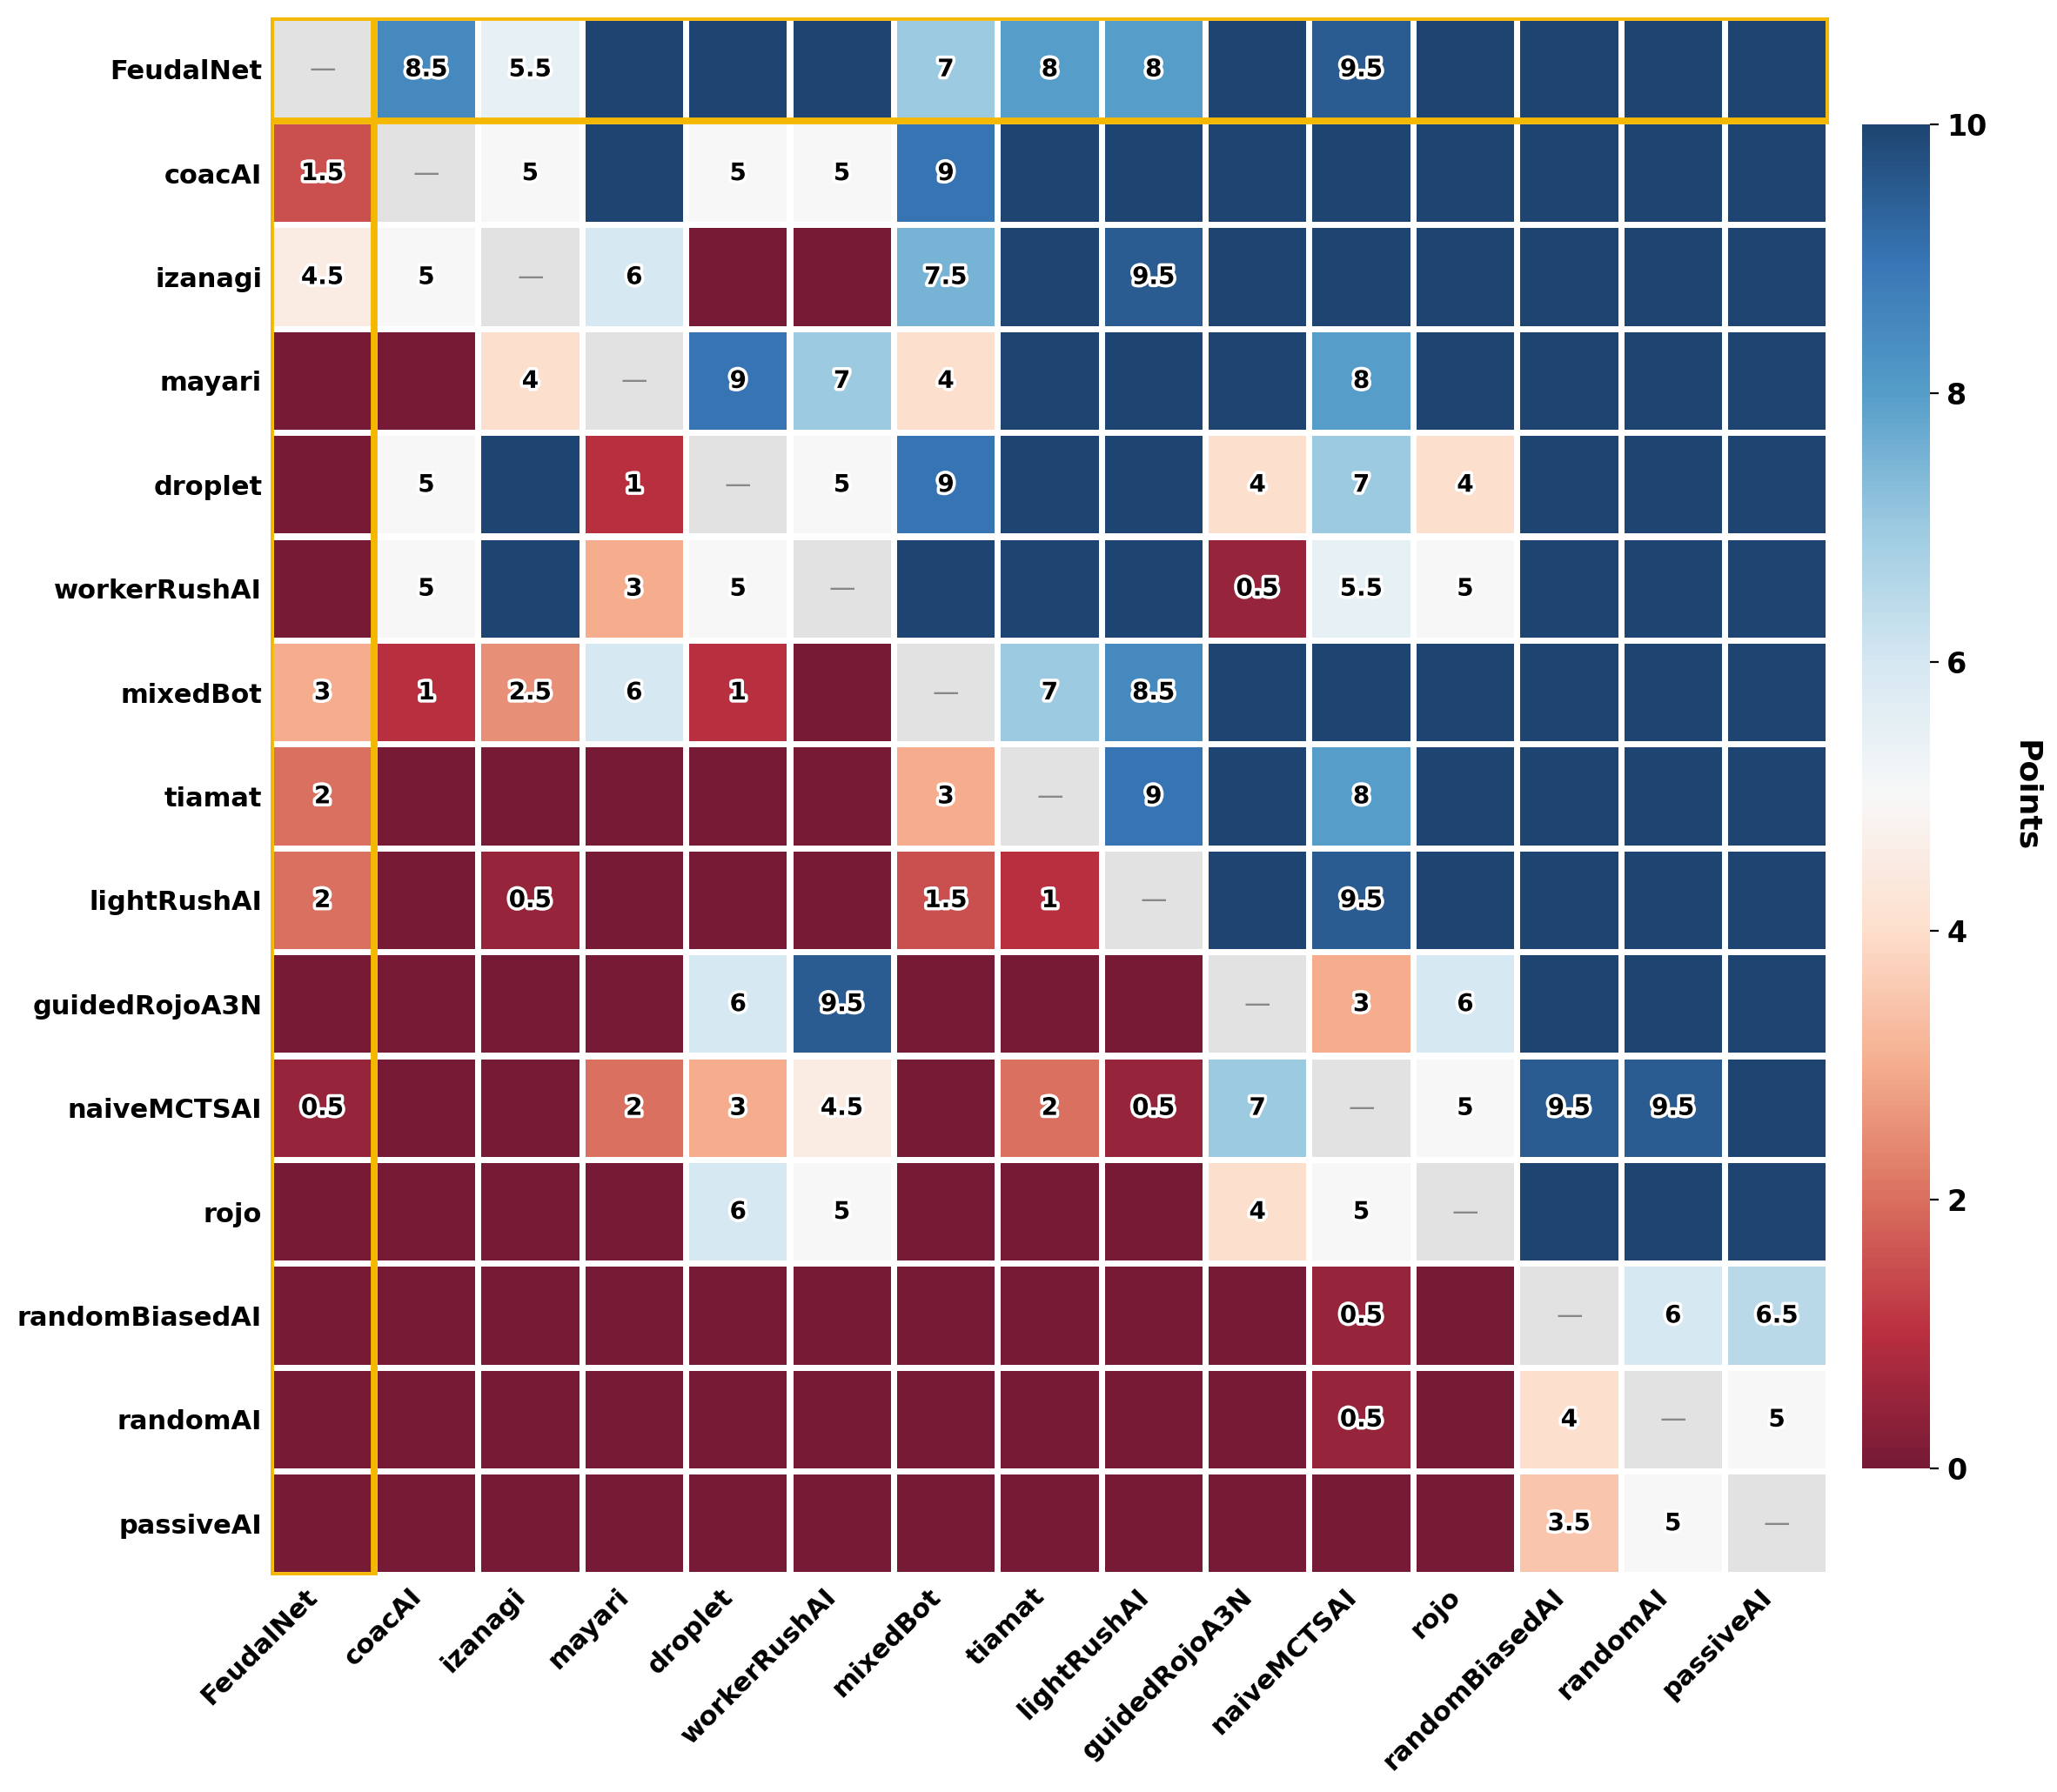
\includegraphics[width=0.45\textwidth]{./round-robin-heatmap-feudal.png}
    \caption{Round-robin tournament results (points per matchup).}\label{fig:round-robin-heatmap-feudal}
\end{figure}

\subsection{Baseline Evaluation}
\label{baseline-eval}

Following the round-robin evaluation, each agent played $1000$ games against every opponent to gather a baseline to begin from.
This was done on both map sizes in batches of $250$ games with different seeds to estimate variance.
The 16$\times$16 results are presented below; the 8$\times$8 results are given in Appendix~B (Figures~\ref{fig:baseline-eval-feudal-8x8} and~\ref{fig:baseline-eval-transformernet-8x8}), where both agents win comfortably against most opponents.

\begin{figure*}
  \centering
  \begin{minipage}[b]{0.48\textwidth}
    \centering
    
\includegraphics[width=\linewidth]{./eval_16x16_feudalnet.pdf}
    \caption{Win-rates achieved by the FeudalNet agent on the 16x16 map.}
    \label{fig:baseline-eval-feudal}
  \end{minipage}
  \hfill
  \begin{minipage}[b]{0.48\textwidth}
    \centering
    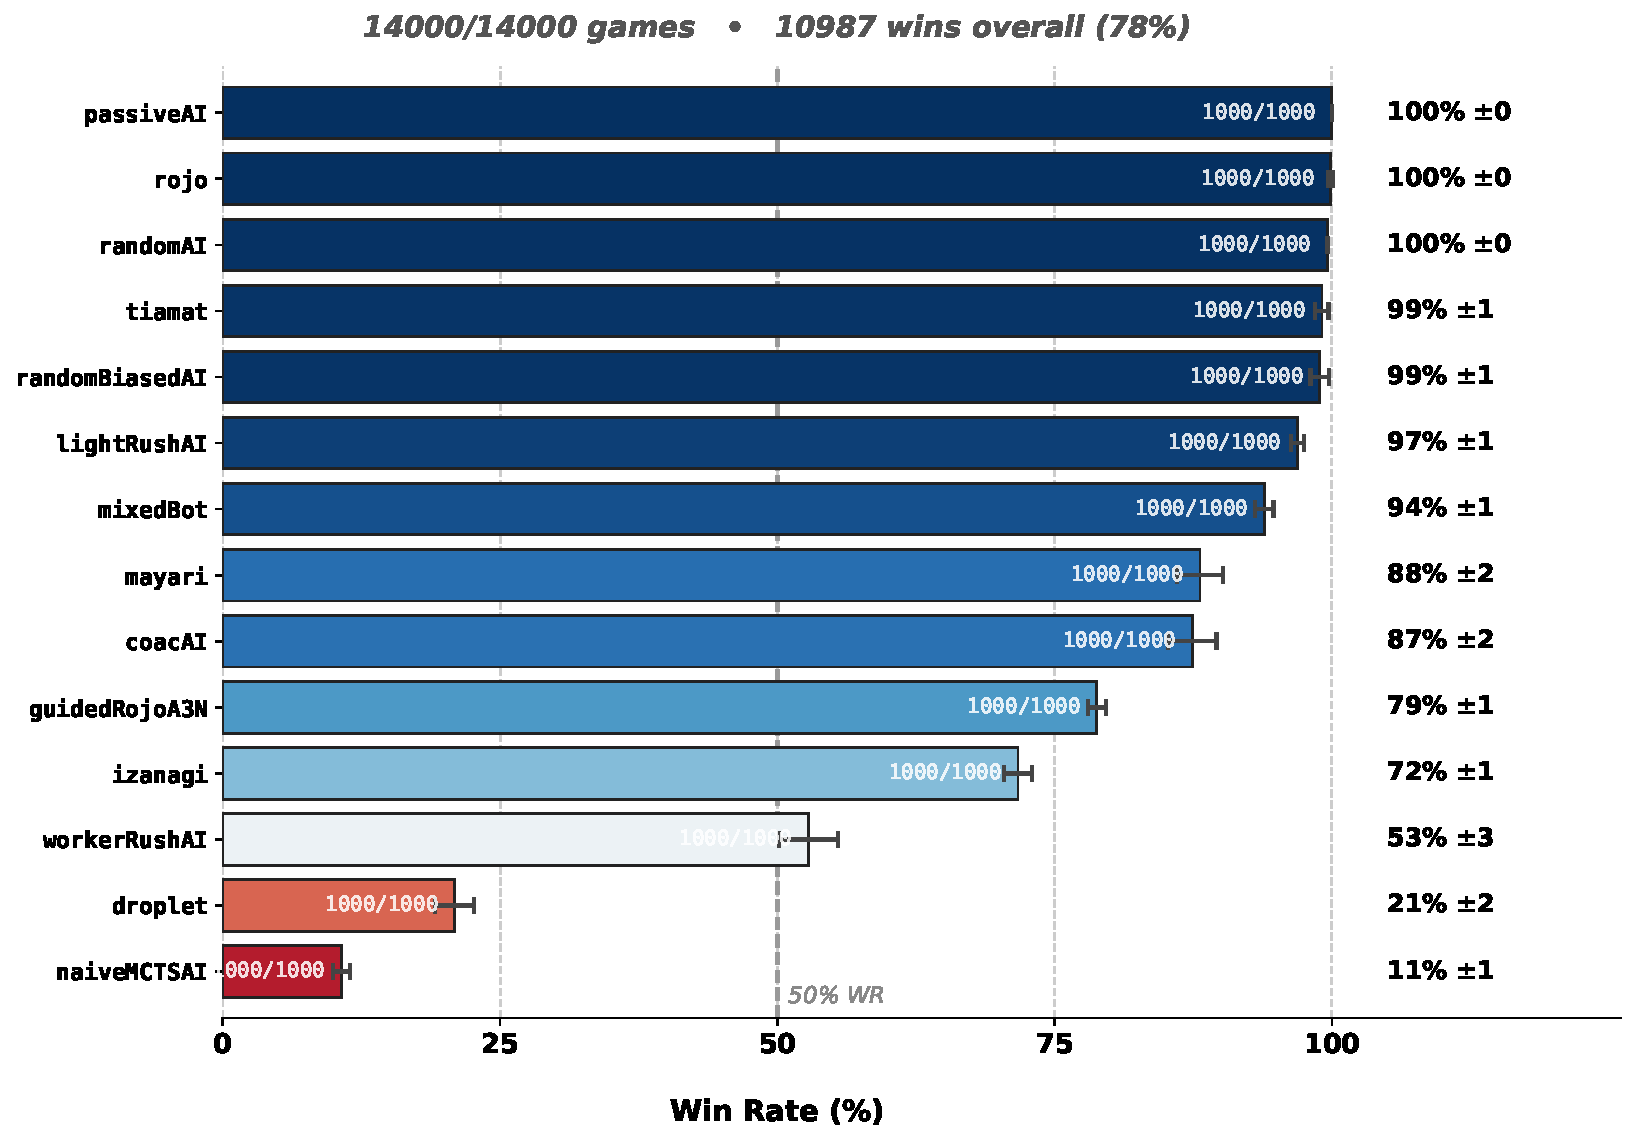
\includegraphics[width=\linewidth]{./eval_16x16_transformernet.pdf}
    \caption{Win-rates achieved by the TransformerNet agent on the 16x16 map.}
    \label{fig:baseline-eval-transformernet}
  \end{minipage}
\end{figure*}


\subsubsection{FeudalNet Results}

The results of this evaluation are graphed in Figure~\ref{fig:baseline-eval-feudal}.

While not a focus of this research, it is clear from the results (Figure~\ref{fig:baseline-eval-feudal}) that our FeudalNet agent is able to confidently score a high win-rate against the majority of the opponents.
Notably, a $99.2\%$ win-rate against the mayari bot and an $88.2\%$ win-rate against the coacAI bot - coacAI is used as a baseline for much of the literature \cite{micrortsgridnet, transformernet}.
However, it struggled significantly against the izanagi bot with a win-rate of $42.8\%$, a figure much lower than the rest of the opponents.

\subsubsection{TransformerNet Results}

The results of this evaluation are graphed in Figure~\ref{fig:baseline-eval-transformernet}.
They align with the original results achieved by Zwingenberger \cite{transformernet}.
Notably, the TransformerNet agent only achieves an $87.4$\% win-rate against the coacAI bot and $88.1$\% against the mayari bot.
Hence, our FeudalNet agent outperforms TransformerNet in the standard \cite{micrortsgridnet, transformernet} evaluations, however FeudalNet clearly struggles against different opponents than TransformerNet - for example, the izanagi matchup.
An outlier in the TransformerNet results is the naiveMCTSAI bot but this win-rate is low due to the sheer number of draws (893 games) achieved in this matchup and was noted by Zwingenberger \cite{transformernet}.

\subsubsection{Opponent Selection}
Applying the selection rules of Section~\ref{adaptation-selection} to these results yields four adaptation opponents: izanagi, naiveMCTSAI, mixedBot and tiamat. 
These are the four weakest FeudalNet matchups outside the training set, spanning win-rates from 42.8\% (izanagi) to 88.6\% (tiamat).

\subsection{FeudalNet Adaptation}
\label{feudalnet-adaptation}

Table~\ref{tab:feudalnet-adaptation} summarises FeudalNet's adaptation against the four unseen opponents.
Each win-rate is measured over 1000 games, played as four repeats of 250 games with different seeds.
$\Delta$ is the change in win-rate in percentage points, and Norm.\ Pts is that change normalised by the available headroom, $\Delta/(1-\mathrm{WR}^{\mathrm{pre}})$.
Steps is the number of environment steps at which the stopping criterion halted adaptation, quantised to the 100k-step evaluation cadence.

\begin{table}[t]
  \caption{FeudalNet adaptation against the four unseen opponents ($n = 1000$ games per condition).}
  \label{tab:feudalnet-adaptation}
  \begin{tabular}{lrrrrr}
    \toprule
    Opponent & WR$^{\mathrm{pre}}$ & WR$^{\mathrm{post}}$
             & $\Delta$ (pts) & Norm.\ Pts & Steps \\
    \midrule
    izanagi     & 42.8\% & 95.5\% & $+52.7$ & $+0.92$ & 400k \\
    mixedBot    & 77.8\% & 96.9\% & $+19.1$ & $+0.86$ & 100k \\
    naiveMCTSAI & 79.0\% & 87.1\% &  $+8.1$ & $+0.39$ & 400k \\
    tiamat      & 88.6\% & 92.8\% &  $+4.2$ & $+0.37$ & 100k \\
    \midrule
    Mean        & 72.1\% & 93.1\% & $+21.0$ & $+0.64$ & --- \\
    \bottomrule
  \end{tabular}
\end{table}


\subsubsection{Statistical Significance of Adaptation Scores}
Table~\ref{tab:feudalnet-significance} reports two-proportion z-tests for each adaptation score ($n = 1000$ games per condition). All four improvements are statistically significant at the 5\% level: the gains against izanagi ($z = 25.5$), mixedBot ($z = 12.9$) and naiveMCTSAI ($z = 4.8$) at $p < 0.001$, and the gain against tiamat ($z = 3.2$, $p = 0.001$) comfortably clearing the threshold despite being the smallest in magnitude ($+4.2$ points). 
Adaptation under the stopping protocol therefore produced measurable improvement against every unseen opponent, and the question the remaining sections address is not whether the agent adapted, but how, and by how much, in each matchup.

\begin{table}[t]
  \caption{Two-proportion z-tests on the FeudalNet adaptation
  scores ($n = 1000$ games per condition). $p$-values are two-sided
  and uncorrected; all four improvements are significant at the
  5\% level.}
  \label{tab:feudalnet-significance}
  \begin{tabular}{lrrrrl}
    \toprule
    Opponent & WR$^{\mathrm{pre}}$ & WR$^{\mathrm{post}}$
             & $\Delta$ (pts) & $z$ & $p$ \\
    \midrule
    izanagi     & 42.8\% & 95.5\% & $+52.7$ & $25.5$ & $<0.001$ \\
    mixedBot    & 77.8\% & 96.9\% & $+19.1$ & $12.9$ & $<0.001$ \\
    naiveMCTSAI & 79.0\% & 87.1\% &  $+8.1$ &  $4.8$ & $<0.001$ \\
    tiamat      & 88.6\% & 92.8\% &  $+4.2$ &  $3.2$ & $0.001$  \\
    \bottomrule
  \end{tabular}
\end{table}


\subsubsection{Raw versus Normalised Adaptation}
Under the final results the two metrics agree on the ordering of the matchups: izanagi shows the largest gain by both raw delta ($+52.7$ points) and normalised points ($+0.92$), followed by mixedBot ($+19.1$, $+0.86$), with naiveMCTSAI ($+8.1$, $+0.39$) and tiamat ($+4.2$, $+0.37$) close together at the bottom. 
Read together, the metrics show that adaptation gains scale with the available headroom: the weaker the baseline matchup, the more the agent improved, both absolutely and as a fraction of what was achievable - with the two hardest baseline matchups recovering over 85\% of their remaining headroom. 
The normalised score does its main work in the cross-agent comparison of Section~\ref{ans-research}, where the agents begin from different baselines against the same opponents and raw deltas alone would favour whichever agent had more room to improve.

\subsubsection{Converting Draws against naiveMCTSAI}
\label{naiveMCTSAI}
The naiveMCTSAI matchup is distinctive in its score line (Win/Loss/Draw). Before adaptation, FeudalNet recorded $790$/$30$/$180$ over 1000 games. 
Outright losses were rare ($3.0\%$) - the deficit in win-rate came almost entirely from draws ($18.0\%$ of games), which our evaluation counts as losses.
The agent was rarely beaten by this opponent - it was failing to close games out within the 2000-tick limit, consistent with the draw counts Zwingenberger~\cite{transformernet} reported for TransformerNet in the same matchup. 
After adaptation the score line becomes $871$/$19$/$110$. 
The draw rate falls from $18.0\%$ to $11.0\%$ and the loss rate from $3.0\%$ to $1.9\%$, so the $+8.1$-point gain is driven almost entirely by games that previously stalled into draws now being completed as wins.
This reading is supported by the win-length statistics. 
Mean steps-to-win is essentially unchanged ($935.1 \pm 229.1$ before adaptation, $934.2 \pm 221.5$ after) despite 81 additional wins - the games the adapted agent now closes out are completed at the same pace as those it already won, rather than being scraped in near the 2000-tick limit. 
This argues that adaptation removed whatever caused games to stall, instead of merely rushing stalled games over the line.

\subsubsection{Counter-Strategy against izanagi}
\label{izanagi-strat}
izanagi was FeudalNet's weakest matchup by a wide margin, with a baseline win-rate of $42.8\%$.
This matchup was also hard in absolute terms, not only specifically for FeudalNet - izanagi placed third in the round-robin tournament (Section~\ref{rr}).
The metrics of the pre-adaptation games show why. 
Draws are negligible ($1.6\%$) and losses are decisive, arriving at a mean of $1307 \pm 249$ ticks - the agent reliably survives the opening but is beaten in the mid-game, well short of the 2000-tick limit.
Adaptation did not merely narrow this gap, it flipped the matchup, lifting the win-rate to $95.5\%$, the largest improvement of the four opponents by both raw delta ($+52.7$ points) and normalised points ($+0.92$).

The game-length statistics in Table~\ref{tab:izanagi-steps} identify how. 
Mean steps-to-win changes from $825 \pm 252$ ticks to $358 \pm 83$, hence the adapted agent ends games in roughly a third of the time, and the tight spread indicates a single, standard plan that directly counters izanagi. 
The adapted agent has discovered an early timing attack that concludes games before the mid-game window in which izanagi previously won ever arrives. 
The remaining losses reinforce this early attack as they now end at $994 \pm 232$ ticks rather than $1307$, signs of a committed early attack that leaves the agent too far behind to recover if failed. 
Notably, this matchup also required the largest adaptation budget, stopping only at 400k steps where mixedBot and tiamat stopped at the first 100k evaluation -  consistent with the gain coming from the discovery of a new strategy rather than refinement of the existing one, which the extra training time was needed to find.

\begin{table}[t]
  \caption{Game-length statistics in ticks for the izanagi matchup before and after adaptation ($n = 1000$ games per condition; draws excluded).}
  \label{tab:izanagi-steps}
  \begin{tabular}{lrrrr}
    \toprule
    & \multicolumn{2}{c}{Before adaptation}
    & \multicolumn{2}{c}{After adaptation} \\
    \cmidrule(lr){2-3} \cmidrule(lr){4-5}
    & Mean ticks & $n$ & Mean ticks & $n$ \\
    \midrule
    Steps to win  &  $824.9 \pm 251.9$ & 428 & $358.3 \pm 82.5$  & 955 \\
    Steps to lose & $1306.5 \pm 248.5$ & 556 & $994.0 \pm 231.6$ &  19 \\
    \bottomrule
  \end{tabular}
\end{table}

\subsubsection{Steps to Threshold}
Adaptation halted at the first 100k-step evaluation for mixedBot and tiamat, while izanagi and naiveMCTSAI trained to 400k steps before stopping. 
Two points of note should be considered from Section~\ref{adaptation-selection} when reading these values. 
First, they are quantised to the 100k evaluation cadence - a stop at the first check means only that the criterion was already satisfied by 100k steps, so these values are upper bounds on the training actually required. 
Second, the stop is triggered by a 50-game screening measurement, not the reported win-rates - the two can disagree, and naiveMCTSAI is the case in point, where the screened stop at 400k verified at $87.1\%$ over 1000 games, short of the $90\%$ threshold.

Read with those points, the split is still informative. 
The two matchups requiring 400k steps are the two that demanded more than refinement of the converged policy. 
izanagi, where the budget was spent discovering a new strategy (Section~\ref{izanagi-strat}), and naiveMCTSAI, where the draw problem was substantially but not fully resolved within it (Section~\ref{naiveMCTSAI}). 
The two stopping at the first check, mixedBot and tiamat, (100k steps) began from the strongest baselines ($88.6\%$ and $77.8\%$) and needed only marginal improvement to satisfy the criterion. 
Steps to threshold therefore tracks the depth of change adaptation had to make, not merely the size of the baseline deficit.

\subsection{TransformerNet Adaptation}
\label{transformernet-adaptation}

Table~\ref{tab:transformernet-adaptation} summarises TransformerNet's adaptation against the same four opponents, with the columns defined as for FeudalNet in Section~\ref{feudalnet-adaptation}.
The normalised score is omitted for tiamat, where it is undefined for a regression from a near-ceiling baseline.
Two stopping outcomes are marked in the table: against mixedBot and tiamat the baseline already exceeded the $90\%$ threshold, so the criterion fired trivially at the first evaluation, and against izanagi and naiveMCTSAI the 1M-step cap was reached without the criterion being satisfied.

\begin{table}[t]
  \caption{TransformerNet adaptation against the four unseen opponents ($n = 1000$ games per condition). $^{*}$baseline already above threshold; $^{\ddagger}$1M-step cap reached.}
  \label{tab:transformernet-adaptation}
  \begin{tabular}{lrrrrl}
    \toprule
    Opponent & WR$^{\mathrm{pre}}$ & WR$^{\mathrm{post}}$
             & $\Delta$ (pts) & Norm.\ Pts & Steps \\
    \midrule
    izanagi     & 71.7\% & 74.7\% &  $+3.0$ & $+0.11$ & 1M$^{\ddagger}$ \\
    mixedBot    & 93.9\% & 95.5\% &  $+1.6$ & $+0.26$ & 100k$^{*}$ \\
    naiveMCTSAI & 10.7\% & 24.6\% & $+13.9$ & $+0.16$ & 1M$^{\ddagger}$ \\
    tiamat      & 99.1\% & 94.6\% &  $-4.5$ & ---     & 100k$^{*}$ \\
    \bottomrule
  \end{tabular}
\end{table}

\subsubsection{Statistical Significance of Adaptation Scores}

Table~\ref{tab:transformernet-significance} reports two-proportion z-tests for each of TransformerNet's adaptation scores ($n = 1000$ games per condition). 
The gain against naiveMCTSAI ($z = 8.2$, $p < 0.001$) is the only statistically significant improvement. 
The changes against izanagi ($z = 1.5$, $p = 0.13$) and mixedBot ($z = 1.6$, $p = 0.11$) are not distinguishable from sampling noise and are not treated as evidence of adaptation. 
The change against tiamat is significant but in the wrong direction - the win-rate fell from $99.1\%$ to $94.6\%$ ($z = -5.8$, $p < 0.001$), the only significant regression observed for either agent. 
Where FeudalNet improved measurably against every unseen opponent, TransformerNet therefore did so against one, held level against two, and declined against one. The remaining subsections examine each outcome in turn, beginning with the two matchups whose baselines already exceeded the stopping threshold, since that threshold plays a role in how the tiamat regression should be read.

\begin{table}[t]
  \caption{Two-proportion z-tests on the TransformerNet adaptation scores ($n = 1000$ games per condition). $p$-values are two-sided and uncorrected.}
  \label{tab:transformernet-significance}
  \begin{tabular}{lrrrrl}
    \toprule
    Opponent & WR$^{\mathrm{pre}}$ & WR$^{\mathrm{post}}$
             & $\Delta$ (pts) & $z$ & $p$ \\
    \midrule
    izanagi     & 71.7\% & 74.7\% &  $+3.0$ &  $1.5$ & $0.13$ \\
    mixedBot    & 93.9\% & 95.5\% &  $+1.6$ &  $1.6$ & $0.11$ \\
    naiveMCTSAI & 10.7\% & 24.6\% & $+13.9$ &  $8.2$ & $<0.001$ \\
    tiamat      & 99.1\% & 94.6\% &  $-4.5$ & $-5.8$ & $<0.001$ \\
    \bottomrule
  \end{tabular}
\end{table}

\subsubsection{Early Threshold Stops against tiamat and mixedBot}

As reported in the previous section, the tiamat and mixedBot baselines already satisfied the stopping criterion, so both matchups received the smallest number of updates of any TransformerNet adaptation. 
Neither offered much headroom to begin with - in tiamat's case only $0.9$ points - and tiamat is also the one matchup in which either agent regressed significantly. The game-length metrics clarify what that regression consists of.
Mean steps-to-win fell from 811 to 627 ticks, mean steps-to-lose rose from 1033 to 1147, and draws remained at zero, indicating an agent that plays more aggressively - closing games faster but losing more often - rather than one that plays worse. 
We therefore read the regression as a snapshot of a policy caught mid-transition, with the stopping threshold halting training 100k steps into a shift toward a faster, higher-variance style. 
Given a larger adaptation budget the new style may well have consolidated back toward the ceiling, but the protocol, never designed for baselines above threshold, did not allow it to.

\subsubsection{Persistent Stalling against naiveMCTSAI}
\label{stalling}
The naiveMCTSAI matchup was the matchup with the most headroom to improve upon ($10.7\%$). 
However, it should be noted that the low win-rate attributed to the baseline reading is solely due to the scoreline of 107 wins, 0 losses and 893 draws. This is a direct consequence of the low rewards given for winning or losing a game, as noted by Zwingenberger~\cite{transformernet}, in which the agent would simply farm the other rewards until the draw timer is met.
This is similar behaviour to that our FeudalNet agent exhibited pre-adaptation and resolved post-adaptation, thus we compare this shared problem directly. Post-adaptation, TransformerNet's draw rate fell from $89.3\%$ of games to $73.0\%$ and its win-rate rose to $24.6\%$, a statistically significant gain of $+13.9$ points and the largest raw improvement it achieved. 
Additionally, wins became faster (1403 ticks to 1230 ticks), similar to the behaviour seen in the tiamat matchup, where the agent played more aggressively.
The same shift also introduced 24 losses where the baseline had none - the cost of a more committal style against an opponent that had previously never beaten it.

Despite this progress, the stalling problem persists. 
Nearly three games in four still end in a draw, the run exhausted the full 1M step budget without approaching the stopping threshold, and the normalised score of $+0.16$ places the gain in proportion - a sixth of the available headroom was recovered. 
The comparison with FeudalNet is telling. Both agents faced a stalling deficit in this matchup, but FeudalNet's was modest ($18.0\%$ draws) and was largely resolved ($11.0\%$), whereas TransformerNet's was near-total and only slightly decreased. 
The normalised scores ($0.16$ against $0.39$) and the resulting win-rates ($24.6\%$ against $87.1\%$) both favour FeudalNet, and it is on these grounds that Section~\ref{ans-research} qualifies the one matchup on which TransformerNet's adaptation score is the larger.

\subsubsection{No Counter-Strategy against izanagi}
TransformerNet began this matchup from a far stronger position than FeudalNet ($71.7\%$ against $42.8\%$, a 29-point head start), yet the run exhausted the full 1M-step budget without approaching the stopping threshold.
The resulting change in win-rate ($+3.0$ points to $74.7\%$) is not statistically significant, but the composition of results shifted beneath it. Draws fell from $14.8\%$ to $10.3\%$ while losses rose from $13.5\%$ to $15.0\%$ - adaptation converted stalled games into roughly equal numbers of wins and losses, so the more committal play seen in every TransformerNet matchup produced no net gain against an opponent that punishes commitment.

The game-length metrics show why this differs from FeudalNet's result against the same opponent. Mean steps-to-win fell from 1114 to 720 ticks, superficially resembling FeudalNet's collapse to 358, but the spread ($\pm 278$ against FeudalNet's $\pm 83$) indicates faster play in general rather than a single repeatable timing attack. 
More tellingly, mean steps-to-lose was essentially unchanged (1300 to 1217 ticks). FeudalNet's discovered strategy moved its losses from 1307 to 994 ticks because it changed when games were decided; TransformerNet is still being beaten by izanagi's mid-game at the same point as before. The agent learned to play the same game faster - it did not find a different strategy to play. 
Across the same protocol and opponent, the flat agent spent two and a half times the training the hierarchy required and gained a small fraction of the improvement.

\subsubsection{Steps to Threshold}
Table~\ref{tab:transformernet-adaptation} shows that TransformerNet did not genuinely reach the stopping threshold on any matchup. Against tiamat and mixedBot the criterion fired at the first evaluation, but trivially - both baselines ($99.1\%$ and $93.9\%$) already exceeded $90\%$, so these stops record that no adaptation was required rather than that any occurred. 
Against izanagi and naiveMCTSAI the runs exhausted the 1M-step cap without satisfying the criterion, verifying at $74.7\%$ and $24.6\%$ respectively.

A sample-efficiency comparison between the agents is therefore only defined on the two matchups where both began below the threshold. 
On izanagi, FeudalNet reached it in 400k steps where TransformerNet failed within 1M; on naiveMCTSAI, FeudalNet's screened stop at 400k verified at $87.1\%$, short of the threshold but far ahead of TransformerNet's $24.6\%$ after the full budget. 
On tiamat and mixedBot no comparison is possible - TransformerNet began above the line and FeudalNet crossed it within 100k - and the apparent parity of the two 100k entries in the table should not be read as equivalent efficiency. 
We note that the stopping protocol was not designed for baselines already above threshold, a case that TransformerNet's published results against tiamat made foreseeable and that a relative criterion would have handled; we return to this in the future work of Section~\ref{conclusions}.

\subsection{Answering the Research Question}
\label{ans-research}
Sections~\ref{feudalnet-adaptation} and~\ref{transformernet-adaptation} established whether each agent adapted. 
In this section we ask which adapted more. 
Table~\ref{tab:agent-comparison} compares the adaptation scores directly, testing each per-opponent difference $\Delta_{\mathrm{F}} - \Delta_{\mathrm{T}}$ with a two-sided z-test on the difference of the two scores, using unpooled variances with $n = 1000$ games per condition for every win-rate. 
FeudalNet's adaptation score is significantly higher on three of the four unseen opponents - izanagi ($+52.7$ against $+3.0$), mixedBot ($+19.1$ against $+1.6$) and tiamat ($+4.2$ against $-4.5$), each at $p < 0.001$. 
TransformerNet's score is significantly higher on naiveMCTSAI ($+13.9$ against $+8.1$, $p = 0.014$).

The naiveMCTSAI exception is where we have to keep note of the normalised score.
Both agents' deficit in that matchup was stalling, and as Section~\ref{stalling} showed, TransformerNet's raw gain is larger precisely because its drawing problem was more severe - it recovered $0.16$ of its available headroom against FeudalNet's $0.39$, and its post-adaptation win-rate ($24.6\%$) remains far below FeudalNet's ($87.1\%$). 
When weighing raw and normalised scores jointly, the exception is real in absolute terms but does not indicate deeper adaptation.

The research question is therefore answered - given a capped adaptation budget, the hierarchical FeudalNet agent improved its win-rate against unseen opponent strategies by more than the flat TransformerNet agent on a significant majority of matchups. 
Two further observations reinforce the verdict. 
First, the stopping behaviour, which Table~\ref{tab:steps-to-threshold} collects for both agents under the 90\% threshold and 1M-step cap, with stops quantised to the 100k evaluation cadence.
FeudalNet trained to the threshold from below on three matchups, in one case by discovering a qualitatively new strategy (Section~\ref{izanagi-strat}), and its one screened stop (naiveMCTSAI, at 400k) verified at $87.1\%$, just short of the threshold.
TransformerNet reached the threshold on none, stopping trivially on the two matchups whose baselines already exceeded it and exhausting the 1M-step cap on the two that did not. 
Second, the magnitude of the difference on the hardest matchups - FeudalNet converted a losing record against izanagi into a near-solved one ($42.8\% \text{ to } 95.5\%$) in 400k steps, while TransformerNet, starting 29 points ahead against the same opponent, gained a non-significant $+3.0$ over 1M.

\begin{table}[t]
  \caption{Environment steps at which adaptation halted, per agent and opponent. $^{*}$baseline already above threshold; $^{\dagger}$screened stop verified below threshold; $^{\ddagger}$1M-step cap reached.}
  \label{tab:steps-to-threshold}
  \begin{tabular}{lll}
    \toprule
    Opponent & FeudalNet & TransformerNet \\
    \midrule
    izanagi     & 400k             & 1M$^{\ddagger}$ \\
    mixedBot    & 100k             & 100k$^{*}$      \\
    naiveMCTSAI & 400k$^{\dagger}$ & 1M$^{\ddagger}$ \\
    tiamat      & 100k             & 100k$^{*}$      \\
    \bottomrule
  \end{tabular}
\end{table}

\begin{table}[t]
  \caption{Per-opponent comparison of adaptation scores, $\Delta_{\mathrm{F}} - \Delta_{\mathrm{T}}$, tested with a two-sided z-test on the difference of the two scores.}
  \label{tab:agent-comparison}
  \begin{tabular}{lrrrrl}
    \toprule
    Opponent & $\Delta_{\mathrm{F}}$ (pts) & $\Delta_{\mathrm{T}}$ (pts)
             & Diff (pts) & $z$ & $p$ \\
    \midrule
    izanagi     & $+52.7$ &  $+3.0$ & $+49.7$ & $19.0$ & $<0.001$ \\
    mixedBot    & $+19.1$ &  $+1.6$ & $+17.5$ & $10.1$ & $<0.001$ \\
    tiamat      &  $+4.2$ &  $-4.5$ &  $+8.7$ &  $5.8$ & $<0.001$ \\
    naiveMCTSAI &  $+8.1$ & $+13.9$ &  $-5.8$ & $-2.5$ & $0.014$  \\
    \bottomrule
  \end{tabular}
\end{table}

\subsection{Robustness of Adaptation as a Property of the Hierarchy}
We consider this the most notable finding of the study, although it was not one we set out to test. 
Our research question asked how much each agent adapted; the process of running the experiments revealed a difference in how reliably they did so. 
FeudalNet reached the stopping threshold against three of four unseen opponents with a handful of hyperparameter changes, fixed once and never revisited.
TransformerNet, by contrast, proved sensitive to nearly every choice made in adapting it, and its one significant gain left the underlying behaviour of the matchup largely intact.

We believe the hierarchy is robust for a simple reason - it keeps apart the pieces that go wrong early in adaptation. 
Three mechanisms stand out. 
First, the critic. 
When an agent meets a new opponent its value estimates are wrong until they re-learn, and any policy update driven by them is driven by noise. FeudalNet's PPG phase retrains the critic on stored hidden states, so the critic can be corrected without touching the policy. 
TransformerNet's critic shares its network with the policy, so the two cannot be separated - correcting one disturbs the other. 
Second, the Worker's learning signal. The Worker also receives a dense intrinsic reward for following the Manager's goal, computed without any value estimate, so part of its learning signal stays reliable while the extrinsic critic recalibrates to the new opponent. 
The Worker therefore always has something sensible to learn from, which keeps its training stable during the period in which the extrinsic advantage cannot be trusted. 
Third, exploration. 
The Manager explores by occasionally trying a new goal, which changes the agent's whole plan at once. 
This is how a genuinely new strategy against izanagi could be found in 400k steps. 
A flat policy explores only by randomising individual unit actions, which produced faster play against izanagi but no new plan in 1M steps.

We note, however, that this comparison involves one hierarchical agent and one flat agent, so differences between them cannot be cleanly attributed to hierarchy itself rather than to the specific design choices of each.
Some of TransformerNet's fragility is incidental rather than inherent to flat policies - notably its shared encoder and the reward weighting its own author identified as inducing reward hacking~\cite{transformernet} - and, following Nachum et al.~\cite{badhrl}, a flat baseline equipped with detached value replay and structured exploration might close the robustness gap.
We leave that test to future work.

\section{Conclusions}
\label{conclusions}

This paper asked whether a hierarchical reinforcement learning agent adapts to unseen opponents in Gym-\textmu RTS more effectively than a flat one. 
To answer it we introduced FeudalNet, a feudal agent that replaces the recurrent memory of FeUdal Networks with transformers operating on two timescales and adds a dedicated opponent-modelling stream, and evaluated it alongside TransformerNet under a common few-shot adaptation protocol against four unseen opponents. FeudalNet proved a strong agent in its own right, winning a round-robin tournament against all fourteen scripted opponents and exceeding TransformerNet on the standard evaluation suite. 
Under adaptation it improved significantly against all four unseen opponents, in one case discovering a new counter-strategy that turned its weakest matchup ($42.8\%$) into a near-solved one ($95.5\%$) within 400k steps. 
TransformerNet improved significantly against one opponent, held level against two, and regressed against one. 
FeudalNet's adaptation score was significantly higher on three of the four matchups, and the research question is answered in the affirmative.

The most notable finding was not the one we set out to test. 
Beyond adapting more, the hierarchy adapted more reliably - reaching the stopping threshold with a handful of hyperparameter changes fixed once, where the flat agent proved sensitive to nearly every choice made in adapting it. 
We attribute this to the hierarchy keeping apart the components that are unreliable early in adaptation - the critic, the low-level learning signal, and exploration - and we regard the robustness of adaptation, rather than its magnitude alone, as the practical advantage of the hierarchical structure this work demonstrates.

\subsection{Future Work}
The robustness finding suggests the most direct next experiment - a flat baseline equipped with the mechanisms we credit for FeudalNet's stability, detached value replay and structured exploration, to test whether the gap is a property of hierarchy or of those components, since a comparison of one hierarchical and one flat agent cannot cleanly separate the two. Comparison against further flat architectures, including the GridNet and UAS agents of Huang et al.~\cite{micrortsgridnet}, would broaden the baseline. 
Each adaptation reported here was a single run per agent and opponent, and since adaptation outcomes in reinforcement learning are known to vary across seeds, multiple adaptation seeds per matchup would quantify the variance the reported scores currently carry.
The stopping criterion, screened on 50 games and undefined for baselines already above the threshold, should be replaced by a relative criterion that handles the two TransformerNet matchups which exposed it.
Finally, all experiments used a single $16{\times}16$ map with the agent playing from one side, so extending the protocol to larger maps, varied layouts, and both starting sides would test whether the adaptation advantage generalises from unseen opponents to unseen environments.

\bibliographystyle{ACM-Reference-Format-etal}
\bibliography{citations}

\clearpage
\appendix

\section{Opponents}

\begin{table}[ht]
\centering
\caption{Built-in microRTS opponent bots used for evaluation. Bots that won a MicroRTS competition are marked with the corresponding year and venue.}
\label{tab:opponent-table}
\begin{tabular}{lc}
\toprule
\textbf{Opponent Name} & \textbf{Competition Winner} \\
\midrule
passiveAI       & --               \\
randomAI        & --               \\
rojo            & --               \\
workerRushAI    & --               \\
mayari          & 2021, 2024 CoG   \\
lightRushAI     & --               \\
coacAI          & 2020 CoG         \\
mixedBot        & --               \\
naiveMCTSAI     & --               \\
izanagi         & --               \\
droplet         & --               \\
guidedRojoA3N   & --               \\
tiamat          & 2018 CoG         \\
randomBiasedAI  & --               \\
\bottomrule
\end{tabular}
\end{table}


\clearpage

\onecolumn
\section{8x8 Map Results}

\begin{figure}[h]
    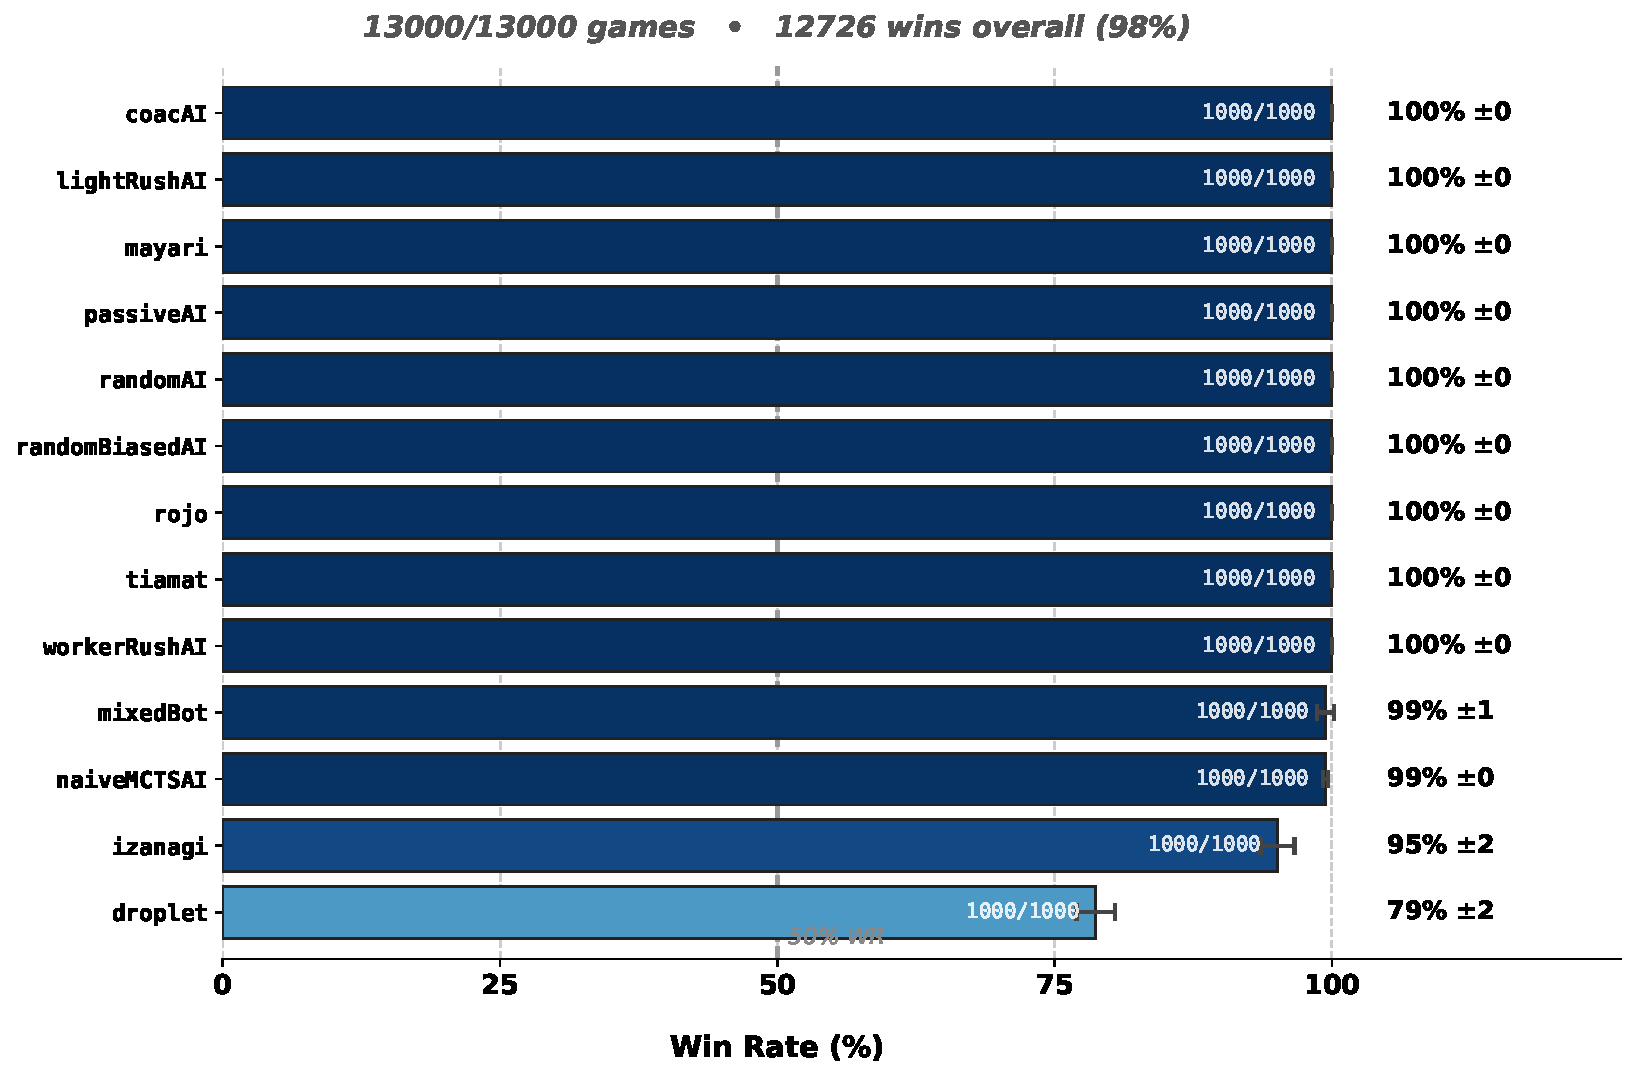
\includegraphics[width=0.75\textwidth]{./eval_8x8_feudal.pdf}
    \caption{Win-rate achieved by the FeudalNet agent on the 8x8 map.}\label{fig:baseline-eval-feudal-8x8}
\end{figure}

\begin{figure}[h]
    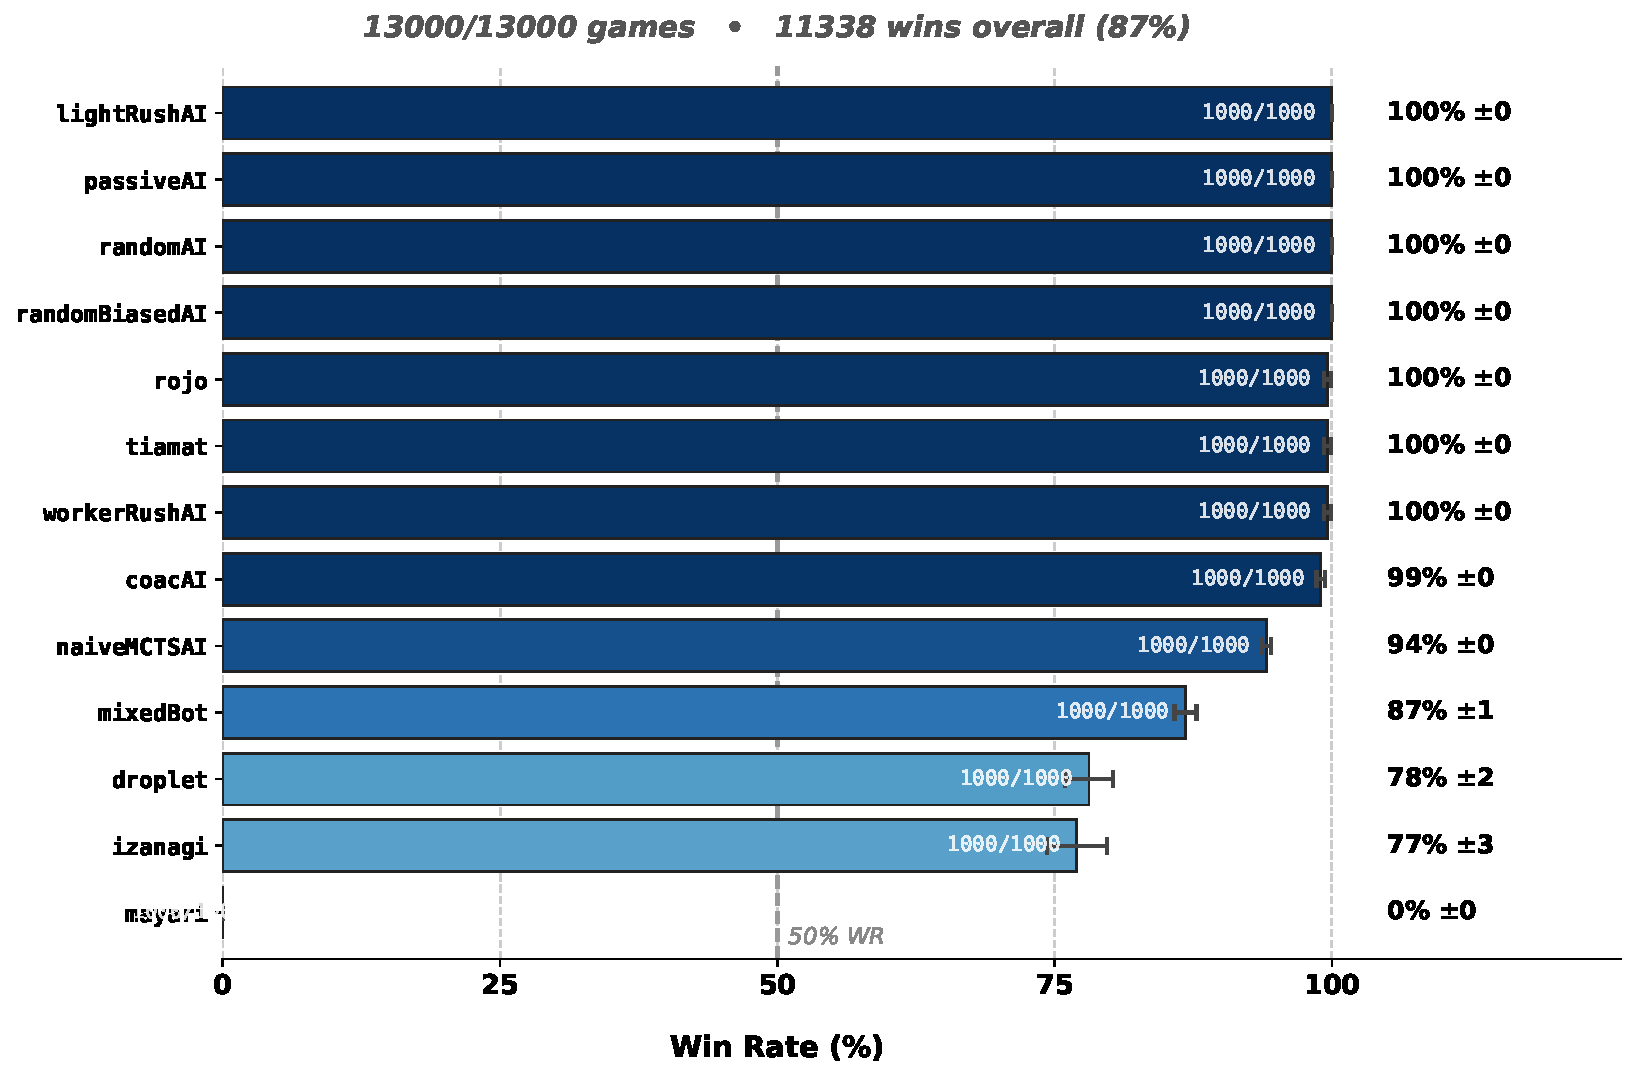
\includegraphics[width=0.75\textwidth]{./eval_8x8_transformer.pdf}
    \caption{Win-rate achieved by the TransformerNet agent on the 8x8 map. Notably it has a 0\% win-rate against mayari.}\label{fig:baseline-eval-transformernet-8x8}
\end{figure}




\clearpage

\begin{table}[ht]
\centering
\caption{Hyperparameters for the FeudalNet agent (16$\times$16 maps).}
\label{tab:hyperparams}
\begin{tabular}{llc}
\toprule
& \textbf{Hyperparameter} & \textbf{Value} \\
\midrule
\textbf{Architecture}
& Input channels                          & 27 \\
& Map size ($H \times W$)                 & $16 \times 16$ \\
& Hidden dimension $d$                    & 128 \\
& Worker attention heads                  & 4 \\
& Worker transformer layers               & 4 \\
& Worker context window $T_W$             & 100 \\
& Manager attention heads                 & 4 \\
& Manager transformer layers              & 6 \\
& Manager context window $T_M$            & 160 \\
& Enemy encoder dimension $d_e$           & 64 \\
& Enemy encoder layers                    & 4 \\
\midrule
\textbf{Training}
& Total environment steps                 & $3 \times 10^{8}$ \\
& Parallel workers                        & 48 \\
& Rollout length                          & 50 \\
& Learning rate                           & $4 \times 10^{-4}$ \\
& Manager time horizon $c$                & 25 \\
& Worker discount $\gamma_W$              & 0.99 \\
& Manager discount $\gamma_M$             & 0.99 \\
& GAE $\lambda$                           & 0.95 \\
& Intrinsic reward weight $\alpha$        & 0.5 \\
& Cosine similarity intrinsic reward      & Yes \\
& Entropy coefficient                     & 0.01 \\
& Value loss coefficient                  & 1.0 \\
& Gradient clip norm                      & 0.5 \\
& Exploration $\epsilon$                  & $10^{-4}$ \\
& PPG policy phases $N_\pi$               & 8 \\
& PPG auxiliary epochs $E_{\text{aux}}$   & 6 \\
\bottomrule
\end{tabular}
\end{table}

\end{document}

